% Options for packages loaded elsewhere
\PassOptionsToPackage{unicode}{hyperref}
\PassOptionsToPackage{hyphens}{url}
%
\documentclass[
]{article}
\usepackage{lmodern}
\usepackage{amssymb,amsmath}
\usepackage{ifxetex,ifluatex}
\ifnum 0\ifxetex 1\fi\ifluatex 1\fi=0 % if pdftex
  \usepackage[T1]{fontenc}
  \usepackage[utf8]{inputenc}
  \usepackage{textcomp} % provide euro and other symbols
\else % if luatex or xetex
  \usepackage{unicode-math}
  \defaultfontfeatures{Scale=MatchLowercase}
  \defaultfontfeatures[\rmfamily]{Ligatures=TeX,Scale=1}
\fi
% Use upquote if available, for straight quotes in verbatim environments
\IfFileExists{upquote.sty}{\usepackage{upquote}}{}
\IfFileExists{microtype.sty}{% use microtype if available
  \usepackage[]{microtype}
  \UseMicrotypeSet[protrusion]{basicmath} % disable protrusion for tt fonts
}{}
\makeatletter
\@ifundefined{KOMAClassName}{% if non-KOMA class
  \IfFileExists{parskip.sty}{%
    \usepackage{parskip}
  }{% else
    \setlength{\parindent}{0pt}
    \setlength{\parskip}{6pt plus 2pt minus 1pt}}
}{% if KOMA class
  \KOMAoptions{parskip=half}}
\makeatother
\usepackage{xcolor}
\IfFileExists{xurl.sty}{\usepackage{xurl}}{} % add URL line breaks if available
\IfFileExists{bookmark.sty}{\usepackage{bookmark}}{\usepackage{hyperref}}
\hypersetup{
  pdftitle={Statistical analysis in RStudio},
  hidelinks,
  pdfcreator={LaTeX via pandoc}}
\urlstyle{same} % disable monospaced font for URLs
\usepackage[margin=1in]{geometry}
\usepackage{longtable,booktabs}
% Correct order of tables after \paragraph or \subparagraph
\usepackage{etoolbox}
\makeatletter
\patchcmd\longtable{\par}{\if@noskipsec\mbox{}\fi\par}{}{}
\makeatother
% Allow footnotes in longtable head/foot
\IfFileExists{footnotehyper.sty}{\usepackage{footnotehyper}}{\usepackage{footnote}}
\makesavenoteenv{longtable}
\usepackage{graphicx,grffile}
\makeatletter
\def\maxwidth{\ifdim\Gin@nat@width>\linewidth\linewidth\else\Gin@nat@width\fi}
\def\maxheight{\ifdim\Gin@nat@height>\textheight\textheight\else\Gin@nat@height\fi}
\makeatother
% Scale images if necessary, so that they will not overflow the page
% margins by default, and it is still possible to overwrite the defaults
% using explicit options in \includegraphics[width, height, ...]{}
\setkeys{Gin}{width=\maxwidth,height=\maxheight,keepaspectratio}
% Set default figure placement to htbp
\makeatletter
\def\fps@figure{htbp}
\makeatother
\setlength{\emergencystretch}{3em} % prevent overfull lines
\providecommand{\tightlist}{%
  \setlength{\itemsep}{0pt}\setlength{\parskip}{0pt}}
\setcounter{secnumdepth}{5}
\usepackage{subfig}

\title{Statistical analysis in RStudio}
\author{}
\date{\vspace{-2.5em}}

\begin{document}
\maketitle

{
\setcounter{tocdepth}{2}
\tableofcontents
}
\hypertarget{abstact}{%
\subsubsection{Abstact}\label{abstact}}

\hypertarget{introduction}{%
\section{INTRODUCTION}\label{introduction}}

The main objective of statistical analysis is to find the correlation
and Trends of seal abundance using the serial dataset.

Firstly we will download the data and convert it into a csv file and
then import data into R studio after importing data We will read the
data and convert the data into data frame Which will import data into
rows and columns. If we check the head of data we can find There are 5
columns 210 observations.

\begin{itemize}
\tightlist
\item
  The first column represents the year, each row consists of the year
  from 2007 to 2010.
\item
  The second column represents the month of a specific year; there are
  15 unique variables if it presents the month of a particular Year.
\item
  The third column represents a site which consists of 7 unique
  variables A,B,C,D,Split and Wall.
\item
  The fourth column represents species which have true unique species
  Harbour and grey.
\item
  The final column represents the average count of each species in a
  particular year year and month each variable has a unique count value.
\end{itemize}

After looking at the column if we check the structure of data,the first
four columns represent the character data type, the last column that is
average count represents the numerical data type.

After getting familiar with the data set ,the first four column data
type should be changed to factor type as in which column the variable of
rows are repetitive.

\begin{longtable}[]{@{}llllr@{}}
\toprule
Summer & Year.Month & Site & Species & average.count\tabularnewline
\midrule
\endhead
summer-2007 & 2007.Jun & A & HARBOUR & 14.1\tabularnewline
summer-2007 & 2007.Jun & B & HARBOUR & 0.3\tabularnewline
summer-2007 & 2007.Jun & C & HARBOUR & 14.7\tabularnewline
summer-2007 & 2007.Jun & Spit & HARBOUR & 0.1\tabularnewline
summer-2007 & 2007.Jun & Wall & HARBOUR & 0.7\tabularnewline
summer-2007 & 2007.Jun & D & HARBOUR & 0.0\tabularnewline
\bottomrule
\end{longtable}

\begin{verbatim}
## 'data.frame':    210 obs. of  5 variables:
##  $ Summer       : chr  "summer-2007" "summer-2007" "summer-2007" "summer-2007" ...
##  $ Year.Month   : chr  "2007.Jun" "2007.Jun" "2007.Jun" "2007.Jun" ...
##  $ Site         : chr  "A" "B" "C" "Spit" ...
##  $ Species      : chr  "HARBOUR" "HARBOUR" "HARBOUR" "HARBOUR" ...
##  $ average.count: num  14.1 0.3 14.7 0.1 0.7 0 0 0.3 0 2.6 ...
\end{verbatim}

\hypertarget{materials-and-methods}{%
\section{MATERIALS AND METHODS}\label{materials-and-methods}}

\hypertarget{qqnorm-test}{%
\subsection{QQNORM Test}\label{qqnorm-test}}

After checking rows and columns of data, it can be easily identified
that only the average.count data column has numerical value. If we check
the normality of the average.count column using the qqnorm()
function,The Below visualization data represents the relationship
between the theoretical and sample quantities which derive the plotted
data is distinctly curved and determines that the data is not normal.

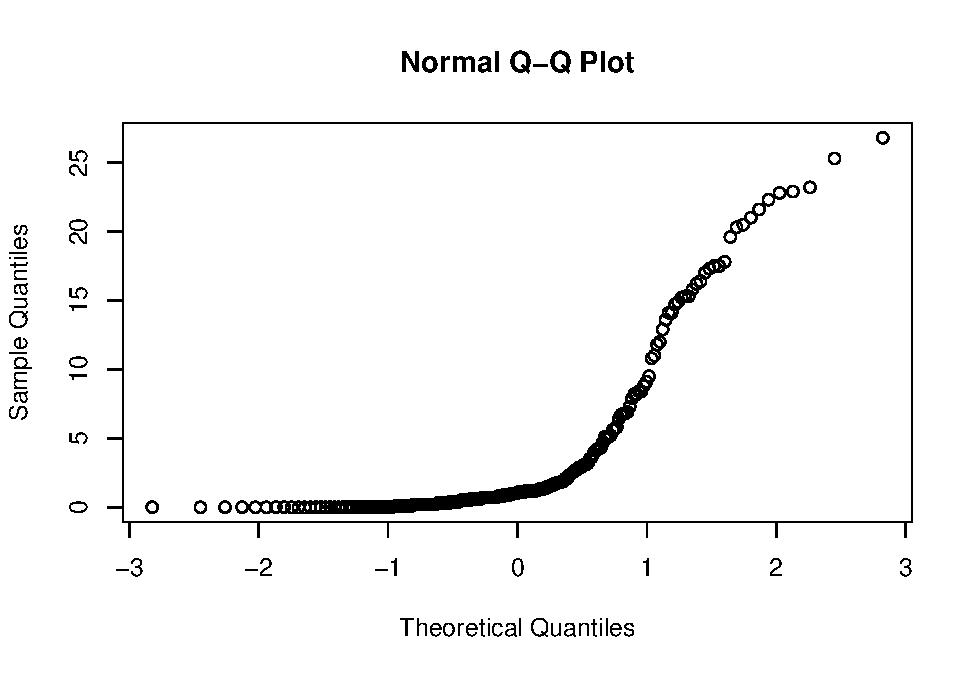
\includegraphics{Statistical-analysis-in-RStudio_files/figure-latex/unnamed-chunk-4-1.pdf}

While finding out that data is not normal in normality test using qqnorm
function, if we run the same test using shapiro.test() function, The
p-value is Greater than 0.01 we can say that it then all hypothesis is
not rejected Data is not significantly distributed therefore we have to
perform non parametric test.

\begin{verbatim}
## 
##  Shapiro-Wilk normality test
## 
## data:  data$average.count
## W = 0.67749, p-value < 2.2e-16
\end{verbatim}

Since the data is not significant,in order to find out The number of
seals are significantly different for each year plot the data of average
count of number of seals for each year but before that we have to change
the data type of the first four columns into factors.

\begin{verbatim}
## 'data.frame':    210 obs. of  5 variables:
##  $ Summer       : Factor w/ 4 levels "2007","2008",..: 1 1 1 1 1 1 1 1 1 1 ...
##  $ Year.Month   : Factor w/ 15 levels "2007.Aug","2007.Jul",..: 3 3 3 3 3 3 3 3 3 3 ...
##  $ Site         : Factor w/ 7 levels "A","B","C","D",..: 1 2 3 6 7 4 5 1 2 3 ...
##  $ Species      : Factor w/ 2 levels "GREY","HARBOUR": 2 2 2 2 2 2 2 1 1 1 ...
##  $ average.count: num  14.1 0.3 14.7 0.1 0.7 0 0 0.3 0 2.6 ...
\end{verbatim}

After changing the data type we can find that the summer column has aur
factor levels, Year. month column has 15 factor levels, the site column
as 7 factor level and and the species column two factor levels.

If we see the data of average count for each year we see that the data
is count is increasing for each year but we cannot that the changes are
significant or not.

In order to find out this we can transfer some non parametric test like
kruskal Wallis rank sum test Which help us to determine the overall
correlation and statistical Association for data by providing a
chi-squared interpretation and a p-value.

But before if we check the below graph, we can see that the 2009 has
highest average count followed by 2010 and the least averge count is
2008.

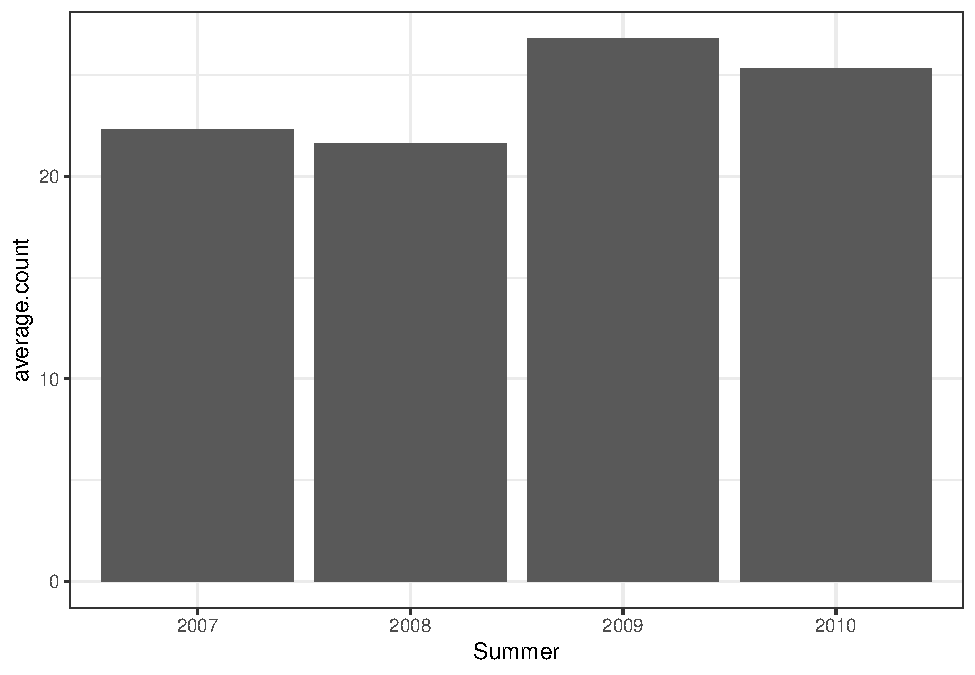
\includegraphics{Statistical-analysis-in-RStudio_files/figure-latex/unnamed-chunk-7-1.pdf}

\hypertarget{kruskal-wallis-test}{%
\subsection{Kruskal-Wallis Test}\label{kruskal-wallis-test}}

In order to perform the Krukals-wallis test, we need to use the
kruskal.test() function.

\begin{verbatim}
## 
##  Kruskal-Wallis rank sum test
## 
## data:  data$average.count and data$Summer
## Kruskal-Wallis chi-squared = 6.236, df = 3, p-value = 0.1007
\end{verbatim}

Firstly, if we explore the overall difference between all the variables
we can see that The P value is greater than 0.01, thus we can say that
it There is no significant difference between the groups. In order to
explore this into more detail to find out that the pairs of groups are
different or not, will use pairwise willox test For comparing different
group levels for multiple testing.

\begin{verbatim}
## 
##  Pairwise comparisons using Wilcoxon rank sum test with continuity correction 
## 
## data:  data$average.count and data$Summer 
## 
##      2007 2008 2009
## 2008 0.89 -    -   
## 2009 0.20 0.43 -   
## 2010 0.43 0.64 0.89
## 
## P value adjustment method: holm
\end{verbatim}

In the above test we can see that the P value for significant years is
quite normal. further, providing an adjustment method we can avoid the
false positive results in order to see more accuracy.

\begin{verbatim}
## 
##  Pairwise comparisons using Wilcoxon rank sum test with continuity correction 
## 
## data:  data$average.count and data$Summer 
## 
##      2007 2008 2009
## 2008 0.54 -    -   
## 2009 0.17 0.17 -   
## 2010 0.17 0.32 0.75
## 
## P value adjustment method: BH
\end{verbatim}

In the above test we can see that the adjusted P value is greater than
0.05, this shows that your value is not significant. In order to
understand it with more clarity if we plot our data we can see that
there was a significant difference between 2010 and 2007, we can see
that the highest number of seals were counted in 2010. Also we can see
that in 2007.

There were some high counts of seal, but in the previous bar graph it
was suggested that there was a big significant difference between 2007
and 2010. From this we can say that the statistical tests were more
accurate and help us to find the significant errors which were present
in data.

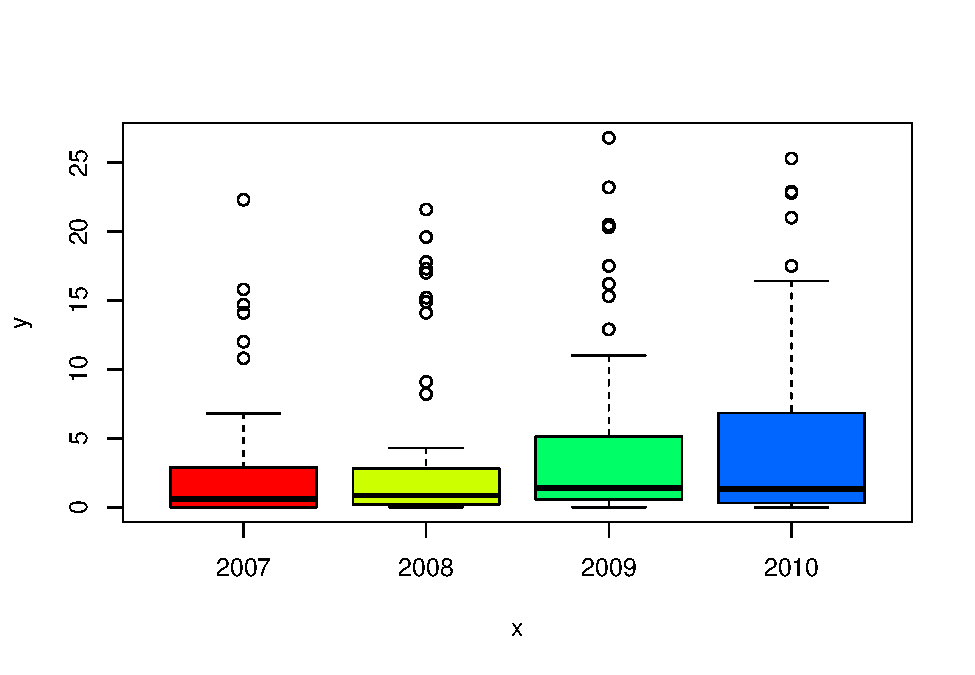
\includegraphics{Statistical-analysis-in-RStudio_files/figure-latex/unnamed-chunk-11-1.pdf}
After this we can check the presence of the seals for each month in a
particular year. We might be able to explore the difference for the
presence of seals in each month of the year.

The plot below shows the values of average count for each month of
particular year.We can see that in 2009 Aug,the number of species were
counted the most and in 2010 Sep the species were counted the least. But
in order to find significant relationship we need to explore the data
and run test accordingly.

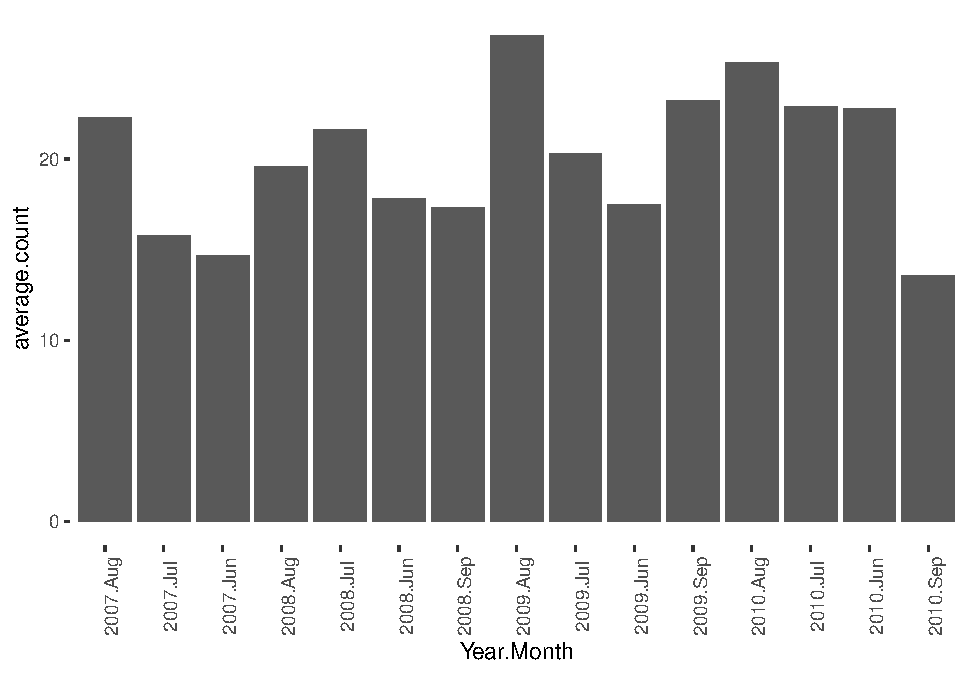
\includegraphics{Statistical-analysis-in-RStudio_files/figure-latex/unnamed-chunk-12-1.pdf}

\hypertarget{kruskal-test-for-each-month}{%
\subsubsection{Kruskal Test For Each
month}\label{kruskal-test-for-each-month}}

If we consider the year 2007, we can see that there is no significant
difference between different months.The p-value is greater than 0.05 and
the adjusted p value is also greater than 0.05.

\begin{verbatim}
## 
##  Kruskal-Wallis rank sum test
## 
## data:  data$average.count[data$Summer == "2007"] and data$Year.Month[data$Summer == "2007"]
## Kruskal-Wallis chi-squared = 1.3113, df = 2, p-value = 0.5191
\end{verbatim}

\begin{verbatim}
## Warning in wilcox.test.default(xi, xj, paired = paired, ...): cannot compute
## exact p-value with ties

## Warning in wilcox.test.default(xi, xj, paired = paired, ...): cannot compute
## exact p-value with ties

## Warning in wilcox.test.default(xi, xj, paired = paired, ...): cannot compute
## exact p-value with ties
\end{verbatim}

\begin{verbatim}
## 
##  Pairwise comparisons using Wilcoxon rank sum test with continuity correction 
## 
## data:  data$average.count[data$Summer == "2007"] and data$Year.Month[data$Summer == "2007"] 
## 
##          2007.Aug 2007.Jul
## 2007.Jul 0.63     -       
## 2007.Jun 0.63     0.63    
## 
## P value adjustment method: BH
\end{verbatim}

If we consider the year 2008, we can see that there is no significant
difference between different months.

\begin{verbatim}
## 
##  Kruskal-Wallis rank sum test
## 
## data:  data$average.count[data$Summer == "2008"] and data$Year.Month[data$Summer == "2008"]
## Kruskal-Wallis chi-squared = 0.86061, df = 3, p-value = 0.8349
\end{verbatim}

\begin{verbatim}
## Warning in wilcox.test.default(xi, xj, paired = paired, ...): cannot compute
## exact p-value with ties

## Warning in wilcox.test.default(xi, xj, paired = paired, ...): cannot compute
## exact p-value with ties

## Warning in wilcox.test.default(xi, xj, paired = paired, ...): cannot compute
## exact p-value with ties

## Warning in wilcox.test.default(xi, xj, paired = paired, ...): cannot compute
## exact p-value with ties

## Warning in wilcox.test.default(xi, xj, paired = paired, ...): cannot compute
## exact p-value with ties

## Warning in wilcox.test.default(xi, xj, paired = paired, ...): cannot compute
## exact p-value with ties
\end{verbatim}

\begin{verbatim}
## 
##  Pairwise comparisons using Wilcoxon rank sum test with continuity correction 
## 
## data:  data$average.count[data$Summer == "2008"] and data$Year.Month[data$Summer == "2008"] 
## 
##          2008.Aug 2008.Jul 2008.Jun
## 2008.Jul 0.93     -        -       
## 2008.Jun 0.93     0.93     -       
## 2008.Sep 0.93     0.93     0.93    
## 
## P value adjustment method: BH
\end{verbatim}

If we consider the year 2007, we can see that there is no significant
difference between different months.

\begin{verbatim}
## 
##  Kruskal-Wallis rank sum test
## 
## data:  data$average.count[data$Summer == "2009"] and data$Year.Month[data$Summer == "2009"]
## Kruskal-Wallis chi-squared = 0.42051, df = 3, p-value = 0.936
\end{verbatim}

\begin{verbatim}
## Warning in wilcox.test.default(xi, xj, paired = paired, ...): cannot compute
## exact p-value with ties

## Warning in wilcox.test.default(xi, xj, paired = paired, ...): cannot compute
## exact p-value with ties

## Warning in wilcox.test.default(xi, xj, paired = paired, ...): cannot compute
## exact p-value with ties

## Warning in wilcox.test.default(xi, xj, paired = paired, ...): cannot compute
## exact p-value with ties

## Warning in wilcox.test.default(xi, xj, paired = paired, ...): cannot compute
## exact p-value with ties

## Warning in wilcox.test.default(xi, xj, paired = paired, ...): cannot compute
## exact p-value with ties
\end{verbatim}

\begin{verbatim}
## 
##  Pairwise comparisons using Wilcoxon rank sum test with continuity correction 
## 
## data:  data$average.count[data$Summer == "2009"] and data$Year.Month[data$Summer == "2009"] 
## 
##          2009.Aug 2009.Jul 2009.Jun
## 2009.Jul 1        -        -       
## 2009.Jun 1        1        -       
## 2009.Sep 1        1        1       
## 
## P value adjustment method: BH
\end{verbatim}

If we consider the year 2010, we can see that there is slight
significant difference between different months.

\begin{verbatim}
## 
##  Kruskal-Wallis rank sum test
## 
## data:  data$average.count[data$Summer == "2010"] and data$Year.Month[data$Summer == "2010"]
## Kruskal-Wallis chi-squared = 2.5001, df = 3, p-value = 0.4753
\end{verbatim}

\begin{verbatim}
## Warning in wilcox.test.default(xi, xj, paired = paired, ...): cannot compute
## exact p-value with ties

## Warning in wilcox.test.default(xi, xj, paired = paired, ...): cannot compute
## exact p-value with ties

## Warning in wilcox.test.default(xi, xj, paired = paired, ...): cannot compute
## exact p-value with ties

## Warning in wilcox.test.default(xi, xj, paired = paired, ...): cannot compute
## exact p-value with ties

## Warning in wilcox.test.default(xi, xj, paired = paired, ...): cannot compute
## exact p-value with ties

## Warning in wilcox.test.default(xi, xj, paired = paired, ...): cannot compute
## exact p-value with ties
\end{verbatim}

\begin{verbatim}
## 
##  Pairwise comparisons using Wilcoxon rank sum test with continuity correction 
## 
## data:  data$average.count[data$Summer == "2010"] and data$Year.Month[data$Summer == "2010"] 
## 
##          2010.Aug 2010.Jul 2010.Jun
## 2010.Jul 0.75     -        -       
## 2010.Jun 0.60     0.96     -       
## 2010.Sep 0.96     0.60     0.60    
## 
## P value adjustment method: BH
\end{verbatim}

\hypertarget{specices-abundance}{%
\subsection{Specices Abundance}\label{specices-abundance}}

Considering the data and previous stats we found that there were no
significant difference for each month but in order to get detailed
information about the species we can check the count of each type of
species and find out the non-significant relationship of the data .

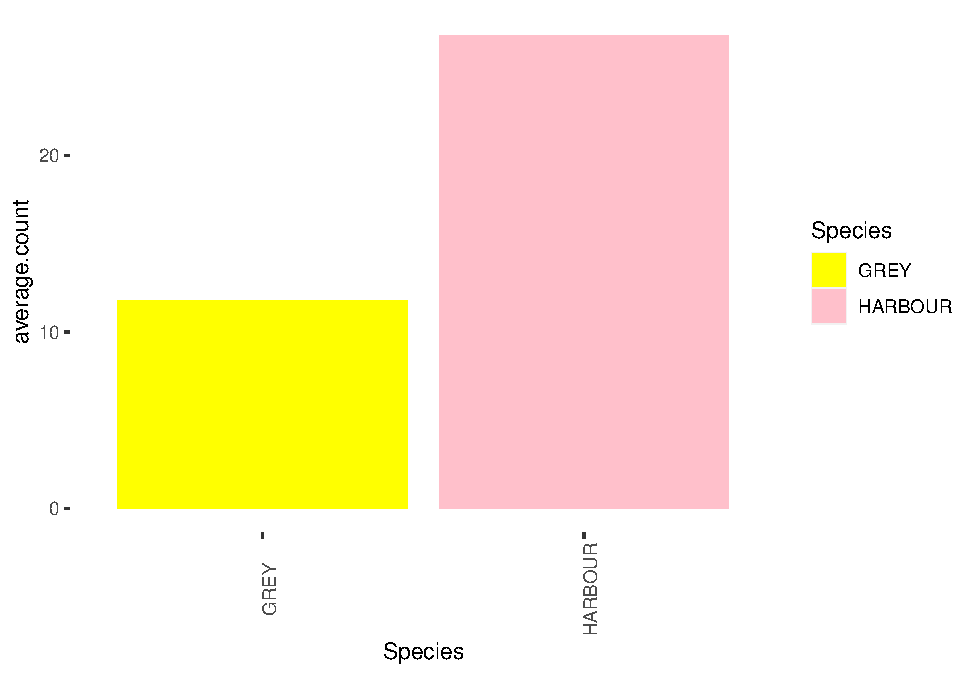
\includegraphics{Statistical-analysis-in-RStudio_files/figure-latex/unnamed-chunk-21-1.pdf}

As we had seen the above graph about the average count is increasing
over year to year, using the kruskal test we can find out the difference
between each species.

\begin{verbatim}
## 
##  Kruskal-Wallis rank sum test
## 
## data:  data$average.count and data$Species
## Kruskal-Wallis chi-squared = 18.66, df = 1, p-value = 1.562e-05
\end{verbatim}

\begin{verbatim}
## 
##  Pairwise comparisons using Wilcoxon rank sum test with continuity correction 
## 
## data:  data$average.count and data$Species 
## 
##         GREY   
## HARBOUR 1.6e-05
## 
## P value adjustment method: BH
\end{verbatim}

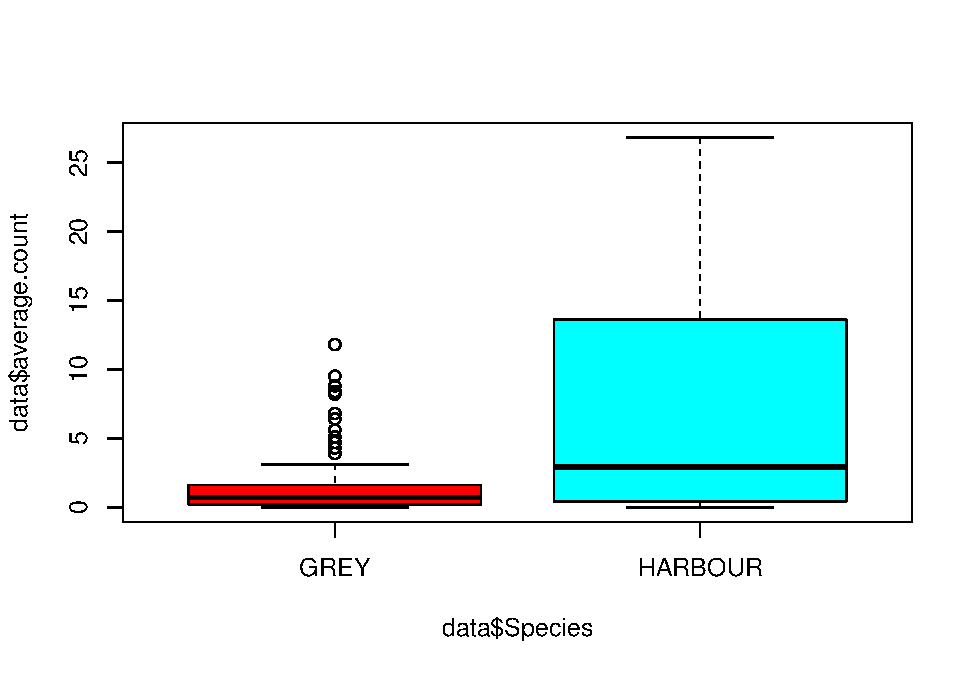
\includegraphics{Statistical-analysis-in-RStudio_files/figure-latex/unnamed-chunk-24-1.pdf}

After performing the test we can easily see the p values is greater than
0.01 and after plotting the below graph we can say that the Harbour
seals population are more comparatively grey. In other way, it can be
derived that the harbor seals are more significantly common than the
grey species.

Also, we can explore data in more detailed way in order to find out
significant difference of species for each year.

If we look at the below stats, we can clearly see the p-value for 2007
year is greater than 0.05 and adjusted p-value is is also greater than
0.05 which derives there is slightest significance difference in the
Species

\begin{verbatim}
## 
##  Kruskal-Wallis rank sum test
## 
## data:  data$average.count[data$Summer == "2007"] and data$Species[data$Summer == "2007"]
## Kruskal-Wallis chi-squared = 3.2976, df = 1, p-value = 0.06938
\end{verbatim}

\begin{verbatim}
## Warning in wilcox.test.default(xi, xj, paired = paired, ...): cannot compute
## exact p-value with ties
\end{verbatim}

\begin{verbatim}
## 
##  Pairwise comparisons using Wilcoxon rank sum test with continuity correction 
## 
## data:  data$average.count[data$Summer == "2007"] and data$Species[data$Summer == "2007"] 
## 
##         GREY 
## HARBOUR 0.071
## 
## P value adjustment method: BH
\end{verbatim}

Again, If we look at the below stats, we can clearly see the p-value for
2008 year is greater than 0.05 and adjusted p-value is is also greater
than 0.05 which derives there is slightest significance difference in
the Species.

\begin{verbatim}
## 
##  Kruskal-Wallis rank sum test
## 
## data:  data$average.count[data$Summer == "2008"] and data$Species[data$Summer == "2008"]
## Kruskal-Wallis chi-squared = 2.727, df = 1, p-value = 0.09866
\end{verbatim}

\begin{verbatim}
## Warning in wilcox.test.default(xi, xj, paired = paired, ...): cannot compute
## exact p-value with ties
\end{verbatim}

\begin{verbatim}
## 
##  Pairwise comparisons using Wilcoxon rank sum test with continuity correction 
## 
## data:  data$average.count[data$Summer == "2008"] and data$Species[data$Summer == "2008"] 
## 
##         GREY
## HARBOUR 0.1 
## 
## P value adjustment method: BH
\end{verbatim}

Again, If we look at the below stats, we can clearly see the p-value for
2009 year is below to 0.05 and adjusted p-value is is also less than
0.05 which derives there is significance difference in the Species.

\begin{verbatim}
## 
##  Kruskal-Wallis rank sum test
## 
## data:  data$average.count[data$Summer == "2009"] and data$Species[data$Summer == "2009"]
## Kruskal-Wallis chi-squared = 10.332, df = 1, p-value = 0.001307
\end{verbatim}

\begin{verbatim}
## Warning in wilcox.test.default(xi, xj, paired = paired, ...): cannot compute
## exact p-value with ties
\end{verbatim}

\begin{verbatim}
## 
##  Pairwise comparisons using Wilcoxon rank sum test with continuity correction 
## 
## data:  data$average.count[data$Summer == "2009"] and data$Species[data$Summer == "2009"] 
## 
##         GREY  
## HARBOUR 0.0013
## 
## P value adjustment method: BH
\end{verbatim}

Finally, If we look at the below stats, we can clearly see the p-value
for 2010 year is below to 0.05 and adjusted p-value is is also less than
0.05 which derives there is significance difference in the Species.

\begin{verbatim}
## 
##  Kruskal-Wallis rank sum test
## 
## data:  data$average.count[data$Summer == "2010"] and data$Species[data$Summer == "2010"]
## Kruskal-Wallis chi-squared = 4.1213, df = 1, p-value = 0.04235
\end{verbatim}

\begin{verbatim}
## Warning in wilcox.test.default(xi, xj, paired = paired, ...): cannot compute
## exact p-value with ties
\end{verbatim}

\begin{verbatim}
## 
##  Pairwise comparisons using Wilcoxon rank sum test with continuity correction 
## 
## data:  data$average.count[data$Summer == "2010"] and data$Species[data$Summer == "2010"] 
## 
##         GREY 
## HARBOUR 0.043
## 
## P value adjustment method: BH
\end{verbatim}

From this we can easily say that in 2007 and 2008 the population of
species were not significantly different where as in 2009 and 2010 we
can say that the population is significantly different from other.

Therefore from here we need to calculate the error in order to find the
out better results and improve the performance but before that we can
check the population of individual species for particular month and
further we can develop the error bars after calculating the error .

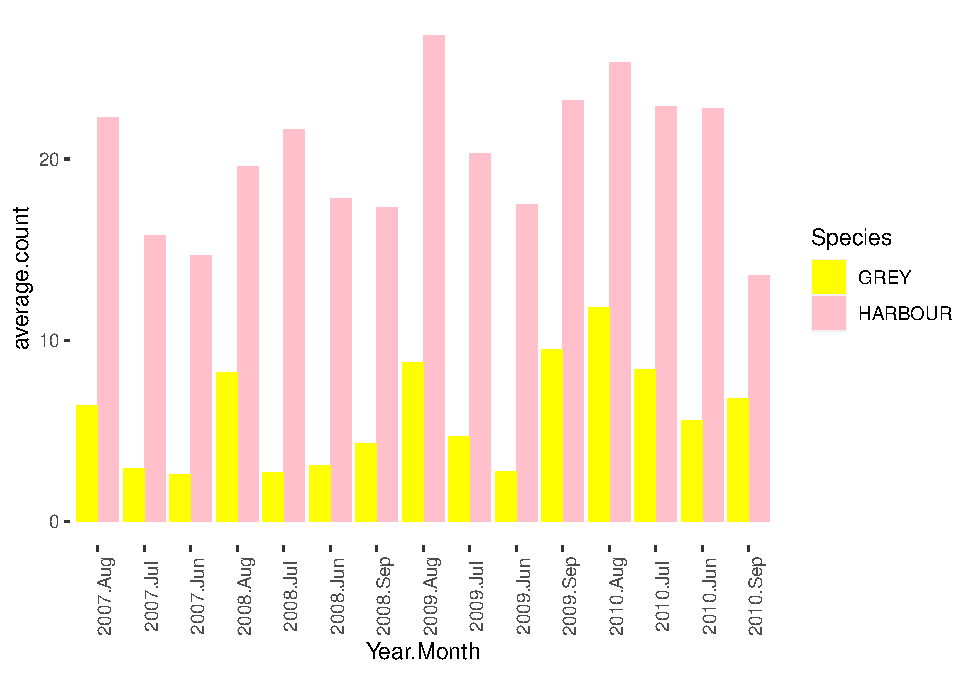
\includegraphics{Statistical-analysis-in-RStudio_files/figure-latex/unnamed-chunk-33-1.pdf}

If you look at the graph of average count of each species in a
particular month everywhere we can see that the existence of herbal
species are way more than the gray species. Therefore we can say that
the herbal species are more common than the gray species.In order to
find the significant differences between the species we need to find the
error species for particular month in each year using SummarySE()
function.

\begin{longtable}[]{@{}llrrrrr@{}}
\toprule
Year.Month & Species & N & average.count & sd & se & ci\tabularnewline
\midrule
\endhead
2007.Aug & GREY & 7 & 1.2857143 & 2.2886885 & 0.8650430 &
2.1166839\tabularnewline
2007.Aug & HARBOUR & 7 & 6.3428571 & 8.2679818 & 3.1250034 &
7.6466079\tabularnewline
2007.Jul & GREY & 7 & 0.8714286 & 1.2051477 & 0.4555030 &
1.1145757\tabularnewline
2007.Jul & HARBOUR & 7 & 5.1714286 & 6.0939080 & 2.3032807 &
5.6359249\tabularnewline
2007.Jun & GREY & 7 & 0.7142857 & 0.9599107 & 0.3628121 &
0.8877693\tabularnewline
2007.Jun & HARBOUR & 7 & 4.2714286 & 6.9254878 & 2.6175883 &
6.4050079\tabularnewline
\bottomrule
\end{longtable}

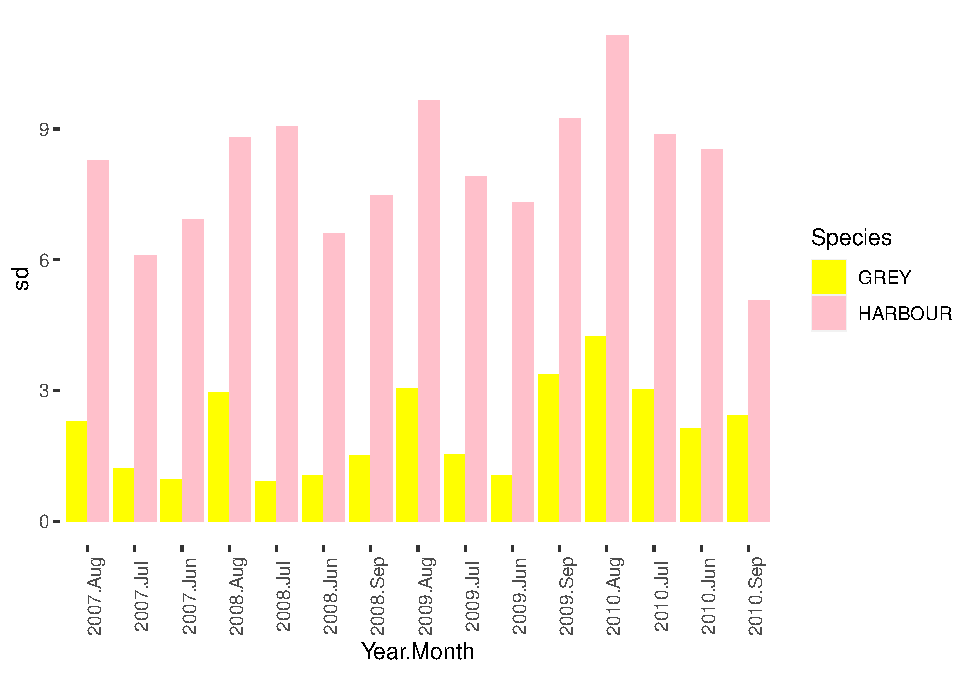
\includegraphics{Statistical-analysis-in-RStudio_files/figure-latex/unnamed-chunk-35-1.pdf}

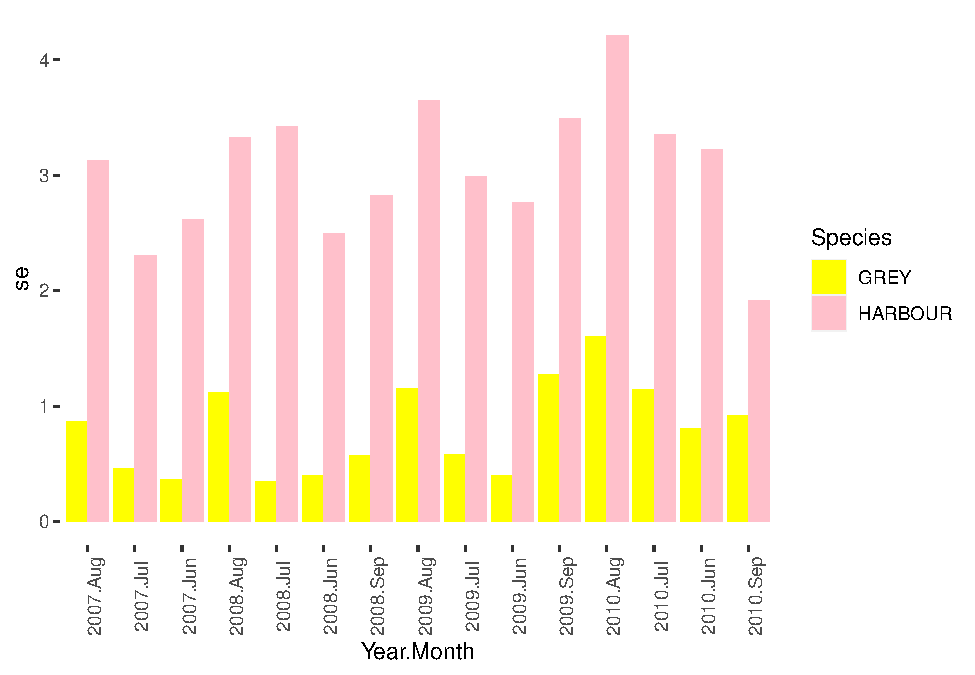
\includegraphics{Statistical-analysis-in-RStudio_files/figure-latex/unnamed-chunk-36-1.pdf}

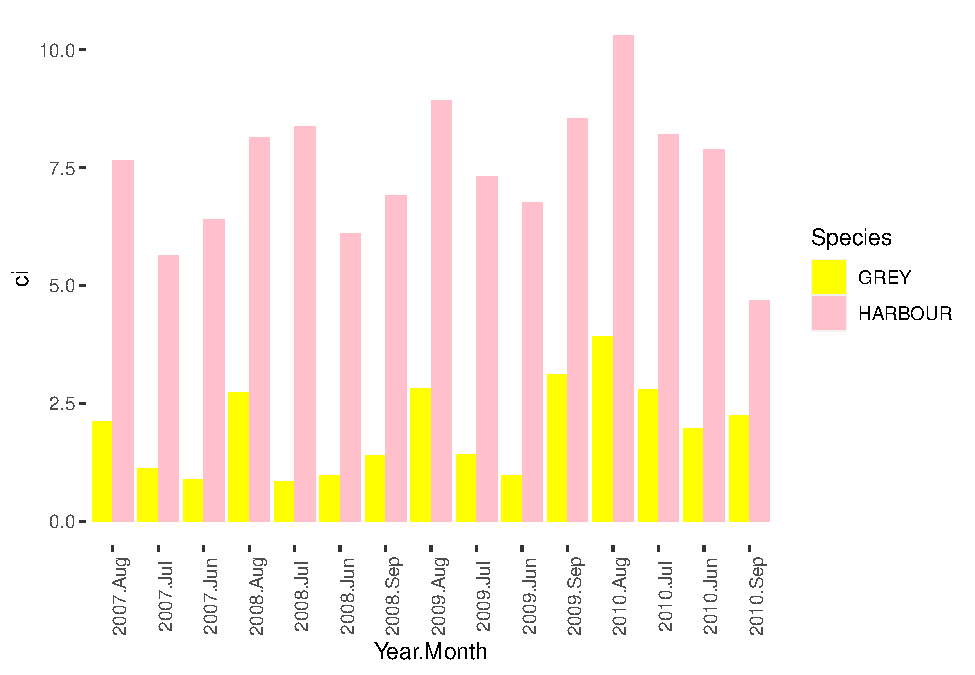
\includegraphics{Statistical-analysis-in-RStudio_files/figure-latex/unnamed-chunk-37-1.pdf}

If we check summary data we can find that the date of it consists of
count, mean, standard deviation, standard error of mean and confidence
interval. in order to find more detailed information we can plot the
significant errors graph using ggplot2 in order to find significant
difference between each species

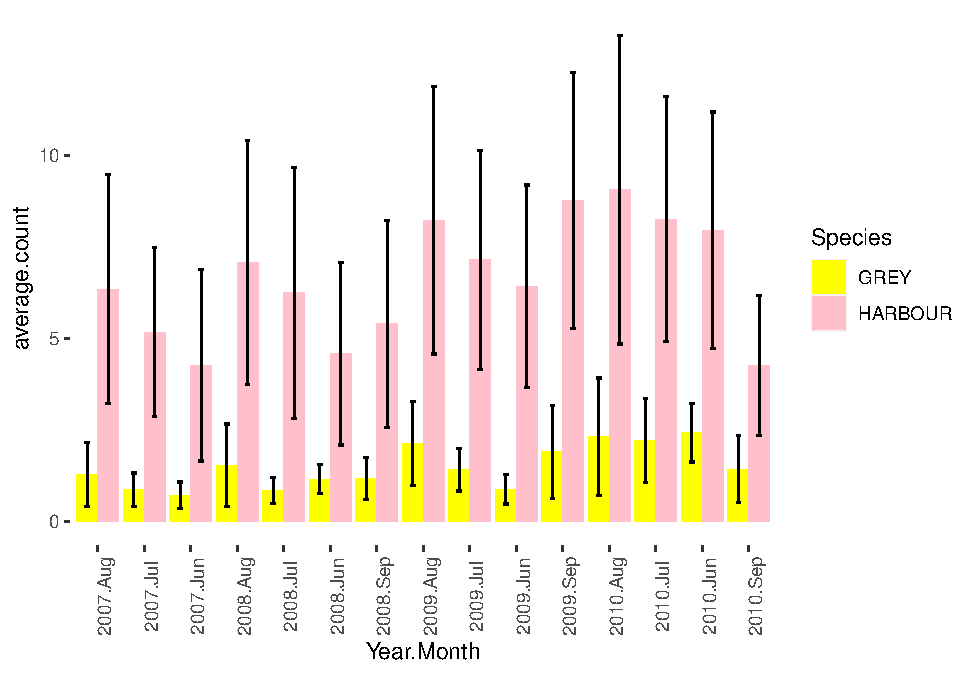
\includegraphics{Statistical-analysis-in-RStudio_files/figure-latex/unnamed-chunk-38-1.pdf}

Considering the above graph clearly shows that the graph provides an
error bar which significantly shows how each species is using standard
error. This clearly signifies difference species for a particular month.

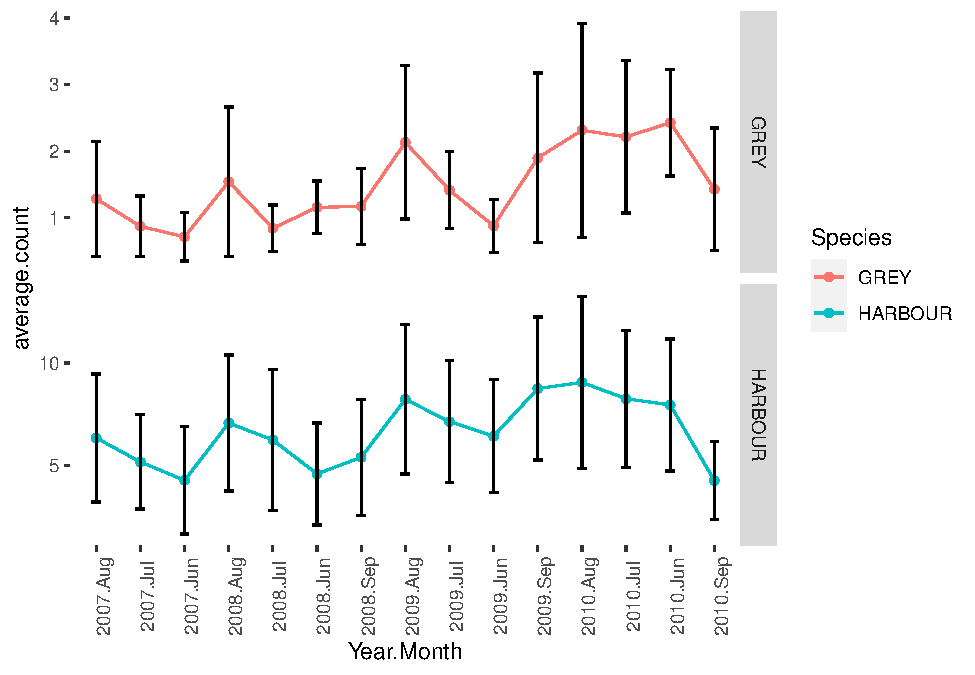
\includegraphics{Statistical-analysis-in-RStudio_files/figure-latex/unnamed-chunk-39-1.pdf}

\hypertarget{results}{%
\section{RESULTS}\label{results}}

In the above test, we have analysed the significant difference between
the species and the count values. We have different nominal variables
and only one measure of variables, however we are able to identify
non-significant values of the population of seals over time.\\
Moreover, when comparing data according to the year wise, we found out
that the highest seal was obtained in 2010 and there were high counts in
summer 2007. But they also found out that the levels of variance in the
data particularly word not explored. Therefore we started exploring data
for each month in a year in order to find out the presence of seals, but
the test suggested that there is no significant difference and different
months for each year. Moreover, Started analysing particular species for
each year. Initially we had seen that the harbour seals species are more
common than grey sea species, after that we found out 2009 and 10 the
data appeared to be more significant 2007 and 2008 the data was slightly
significant. After that, we calculated the standard error, and
visualised the data which represented how the variables are using
standard errors.

By summing up, we can say that the data is well explored, analysed and
ready to be processed for modelling which will help to give better
results for prediction.

\hypertarget{discussion}{%
\section{DISCUSSION}\label{discussion}}

In the above data, We were able to successfully explore and analyse and
find out the normality distribution of existence for both the species.
According to the non parametric test, the most common use of Kruskal
Wallis Test is when the data has one nominal variable and one
measurement variable but test does not assume that a data han is well
distributed and completely align for two parameters which can be mean
and standard deviation and also it is called as one way
anova(Biostathandbook, One Way Annovas). also this test assumes that the
null hypothesis of mean groups are same. therefore if distribution
groups are same, the Kruskal wallis test will not show a significant
difference in their distribution. Yet, the test does not considered that
the data are normally distributed, which can be a big advantage but 800
data has different groups different variants the test will give
inaccurate result. Therefore, if the distribution is different and
variant is different we can use anova test for accurate results

\hypertarget{references}{%
\subsubsection{REFERENCES}\label{references}}

The Kruskal-Wallis One-way Ananysis of Variance by Ranks --Analysis of
k-Between-Group Data with a Quantitative Response Variable. Available
from : \url{https://psych.unl.edu/psycrs/handcomp/hckw.PDF}. {[}Accessed
at 20th December 2020{]} Biostathandbook.com,
\url{http://www.biostathandbook.com/kruskalwallis.html} {[}Accessed at
23d December 2020{]}

\end{document}
